\documentclass[aspectratio=169,11pt]{beamer}
\usetheme{default}
\setbeamertemplate{navigation symbols}{}
\setbeamertemplate{footline}{%
  \hfill\insertframenumber/\inserttotalframenumber\hspace*{4pt}\vspace{2pt}%
}
\usepackage{lmodern}
\usepackage[most]{tcolorbox}
\usepackage{listings}
\usepackage{tikz}
\usetikzlibrary{arrows.meta,positioning,shapes.geometric,fit,backgrounds,shapes.misc}
\usepackage{booktabs}
\usepackage{hyperref}

\definecolor{lcgreen}{HTML}{2E7D32}
\definecolor{lcblue}{HTML}{1565C0}
\definecolor{lcorange}{HTML}{EF6C00}
\definecolor{lcred}{HTML}{C62828}
\definecolor{codebg}{HTML}{F5F5F5}
\definecolor{docgray}{gray}{0.55}

\newtcolorbox{conceptbox}[1][]{colback=yellow!20,colframe=yellow!60!black,title=#1,fonttitle=\bfseries}
\newtcolorbox{warningbox}[1][]{colback=red!15,colframe=red!60!black,title=#1,fonttitle=\bfseries}
\newtcolorbox{tipbox}[1][]{colback=green!10,colframe=green!50!black,title=#1,fonttitle=\bfseries}
\newtcolorbox{codebox}[1][]{colback=blue!10,colframe=blue!40!black,title=#1,fonttitle=\bfseries}

\lstset{
  basicstyle=\ttfamily\scriptsize,
  backgroundcolor=\color{codebg},
  breaklines=true,
  frame=single,
  rulecolor=\color{blue!40!black},
  keywordstyle=\color{lcblue}\bfseries,
  stringstyle=\color{lcgreen},
  commentstyle=\color{docgray}\itshape,
  language=Python,
  showstringspaces=false,
  tabsize=2,
  xleftmargin=2pt,
  xrightmargin=2pt,
}

\newcommand{\docref}[1]{{\scriptsize\color{docgray}[Docs: #1]}}

\title[LangChain Section 01]{Chat Models \& Prompt Templates}
\subtitle{LangChain v1.2.x (March 2026)}
\author[LangChain Slides]{Comprehensive Guide}
\date{\today}

\begin{document}

% ============================================================================
% TITLE SLIDE
% ============================================================================
\begin{frame}
  \titlepage
\end{frame}

% ============================================================================
% OUTLINE
% ============================================================================
\begin{frame}{What We'll Cover}
  \tableofcontents
\end{frame}

% ============================================================================
% SECTION 1: MENTAL MODEL
% ============================================================================
\section{Mental Model: Where Chat Models Fit}

\begin{frame}{LangChain Pipeline Overview}
  \begin{center}
    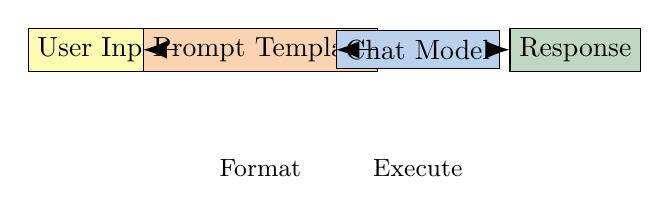
\begin{tikzpicture}[node distance=2cm, auto]
      % Nodes
      \node[draw, rectangle, fill=yellow!30] (input) {User Input};
      \node[draw, rectangle, fill=lcorange!30, right of=input] (prompt) {Prompt Template};
      \node[draw, rectangle, fill=lcblue!30, right of=prompt] (model) {Chat Model};
      \node[draw, rectangle, fill=lcgreen!30, right of=model] (output) {Response};

      % Arrows
      \draw[-{Latex[length=3mm]}] (input) -- (prompt);
      \draw[-{Latex[length=3mm]}] (prompt) -- (model);
      \draw[-{Latex[length=3mm]}] (model) -- (output);

      % Annotations
      \node[below of=prompt, yshift=0.5cm] {\small Format};
      \node[below of=model, yshift=0.5cm] {\small Execute};
    \end{tikzpicture}
  \end{center}

  \begin{conceptbox}[Key Insight]
    Prompt Templates prepare input → Chat Models execute it → You get output.
    This section covers both components in depth.
  \end{conceptbox}
\end{frame}

% ============================================================================
% SECTION 2: MESSAGE TYPES
% ============================================================================
\section{Message Types}

\begin{frame}[fragile]{Message Types: The Foundation}
  \begin{conceptbox}[Core Message Types in LangChain]
    Every chat interaction uses typed messages. This prevents mistakes and enables structured handling.
  \end{conceptbox}

  \begin{itemize}
    \item \textbf{HumanMessage}: User input
    \item \textbf{AIMessage}: Model responses
    \item \textbf{SystemMessage}: Instructions/context for the model
    \item \textbf{ToolMessage}: Results from tool calls
  \end{itemize}

  \docref{langchain.schema}
\end{frame}

\begin{frame}[fragile]{HumanMessage \& AIMessage}
  \begin{codebox}[Basic Messages]
    \begin{lstlisting}
from langchain.schema import HumanMessage, AIMessage

# User speaks
msg1 = HumanMessage(content="What's 2+2?")

# Model responds
msg2 = AIMessage(content="The answer is 4.")

# Use in conversation
messages = [msg1, msg2]
    \end{lstlisting}
  \end{codebox}

  \vspace{0.5cm}
  \begin{tipbox}[Convention]
    Always wrap user input in \texttt{HumanMessage}. This makes intent explicit.
  \end{tipbox}
\end{frame}

\begin{frame}[fragile]{SystemMessage \& ToolMessage}
  \begin{codebox}[Specialized Messages]
    \begin{lstlisting}
from langchain.schema import SystemMessage, ToolMessage

# System: Tells model how to behave
sys = SystemMessage(
    content="You are a helpful math tutor."
)

# Tool: Response from external call
tool_result = ToolMessage(
    content="Result from calculation tool",
    tool_call_id="call_123"
)

messages = [sys, HumanMessage(...), tool_result]
    \end{lstlisting}
  \end{codebox}

  \vspace{0.5cm}
  \begin{warningbox}[Message Order]
    SystemMessage should come \textbf{first} in most cases. Models expect this order.
  \end{warningbox}
\end{frame}

% ============================================================================
% SECTION 3: CHAT MODEL INTERFACE
% ============================================================================
\section{Chat Model Interface}

\begin{frame}{ChatModel Methods}
  \begin{conceptbox}[Core Interface]
    All LangChain chat models follow this pattern: \texttt{invoke} | \texttt{batch} | \texttt{stream} | async versions
  \end{conceptbox}

  \begin{itemize}
    \item \textbf{invoke()}: Single request, wait for response
    \item \textbf{batch()}: Multiple requests at once
    \item \textbf{stream()}: Real-time token streaming
    \item \textbf{ainvoke()}: Async single request
    \item \textbf{abatch()}: Async batch requests
    \item \textbf{astream()}: Async token streaming
  \end{itemize}

  \docref{langchain.chat\_models.base}
\end{frame}

\begin{frame}[fragile]{invoke() - Single Call}
  \begin{codebox}[Basic invoke() Pattern]
    \begin{lstlisting}
from langchain_openai import ChatOpenAI
from langchain.schema import HumanMessage

model = ChatOpenAI(model="gpt-4")

# Single request
message = HumanMessage(content="Hello!")
response = model.invoke([message])

print(response.content)  # "Hello! How can I help?"
    \end{lstlisting}
  \end{codebox}

  \vspace{0.5cm}
  \begin{tipbox}[Note]
    \texttt{invoke()} blocks until the model responds. Use for simple scripts.
  \end{tipbox}
\end{frame}

\begin{frame}[fragile]{batch() - Multiple Calls}
  \begin{codebox}[Batch Processing]
    \begin{lstlisting}
# Process multiple messages at once
messages_batch = [
    [HumanMessage(content="What is AI?")],
    [HumanMessage(content="What is ML?")],
    [HumanMessage(content="What is DL?")]
]

responses = model.batch(messages_batch)

for resp in responses:
    print(resp.content)
    \end{lstlisting}
  \end{codebox}

  \vspace{0.5cm}
  \begin{tipbox}[Efficiency]
    \texttt{batch()} is faster than sequential \texttt{invoke()} calls.
  \end{tipbox}
\end{frame}

% ============================================================================
% SECTION 4: PROVIDER SETUP
% ============================================================================
\section{Provider Setup}

\begin{frame}[fragile]{ChatOpenAI Setup}
  \begin{codebox}[OpenAI Configuration]
    \begin{lstlisting}
from langchain_openai import ChatOpenAI

# Basic setup (uses OPENAI_API_KEY env var)
model = ChatOpenAI(
    model="gpt-4",
    temperature=0.7,
    api_key="sk-..."  # or use env var
)

# For gpt-3.5-turbo
model = ChatOpenAI(model="gpt-3.5-turbo")
    \end{lstlisting}
  \end{codebox}

  \docref{langchain\_openai.ChatOpenAI}
\end{frame}

\begin{frame}[fragile]{ChatAnthropic Setup}
  \begin{codebox}[Anthropic Claude Configuration]
    \begin{lstlisting}
from langchain_anthropic import ChatAnthropic

model = ChatAnthropic(
    model="claude-3-sonnet-20250219",
    temperature=0.7,
    api_key="sk-ant-..."  # or ANTHROPIC_API_KEY
)

# For Claude 3.5 Sonnet
model = ChatAnthropic(
    model="claude-3-5-sonnet-20241022"
)
    \end{lstlisting}
  \end{codebox}

  \docref{langchain\_anthropic.ChatAnthropic}
\end{frame}

\begin{frame}[fragile]{ChatGoogleGenerativeAI Setup}
  \begin{codebox}[Google Gemini Configuration]
    \begin{lstlisting}
from langchain_google_genai import ChatGoogleGenerativeAI

model = ChatGoogleGenerativeAI(
    model="gemini-2.0-flash",
    temperature=0.7,
    api_key="AIzaSy..."  # or GOOGLE_API_KEY
)

# Alternative: gemini-1.5-pro
model = ChatGoogleGenerativeAI(
    model="gemini-1.5-pro"
)
    \end{lstlisting}
  \end{codebox}

  \docref{langchain\_google\_genai.ChatGoogleGenerativeAI}
\end{frame}

\begin{frame}[fragile]{ChatOllama Setup (Local)}
  \begin{codebox}[Ollama Local Model]
    \begin{lstlisting}
from langchain_ollama import ChatOllama

# Requires: ollama pull llama2
model = ChatOllama(
    model="llama2",
    base_url="http://localhost:11434"
)

# For Mistral
model = ChatOllama(model="mistral")

# Streaming enabled by default
response = model.invoke([HumanMessage(...)])
    \end{lstlisting}
  \end{codebox}

  \begin{tipbox}[Local Development]
    Perfect for testing without API costs. Install Ollama from ollama.ai
  \end{tipbox}
\end{frame}

% ============================================================================
% SECTION 5: MODEL PARAMETERS
% ============================================================================
\section{Model Parameters}

\begin{frame}{Key Model Parameters}
  \begin{conceptbox}[Parameters Shape Behavior]
    These parameters control output quality, diversity, and constraints.
  \end{conceptbox}

  \begin{description}
    \item[temperature] Randomness (0.0-2.0). Low = focused, High = creative
    \item[max\_tokens] Output length limit. Plan for input + output
    \item[top\_p] Nucleus sampling (0.0-1.0). Filters unlikely tokens
    \item[model] Which model to use (required)
    \item[stop] List of strings that end generation early
  \end{description}

  \docref{Chat Model Parameters}
\end{frame}

\begin{frame}[fragile]{Temperature \& max\_tokens}
  \begin{codebox}[Common Parameters]
    \begin{lstlisting}
from langchain_openai import ChatOpenAI

# Focused, deterministic (for tasks)
model_task = ChatOpenAI(
    model="gpt-4",
    temperature=0.0,  # No randomness
    max_tokens=200    # Keep output short
)

# Creative (for brainstorming)
model_creative = ChatOpenAI(
    model="gpt-4",
    temperature=1.2,  # More diverse
    max_tokens=1000
)
    \end{lstlisting}
  \end{codebox}

  \vspace{0.5cm}
  \begin{warningbox}[Token Budget]
    \texttt{max\_tokens} includes output only. Ensure input + max\_tokens fits model limit.
  \end{warningbox}
\end{frame}

\begin{frame}[fragile]{Stop Sequences \& top\_p}
  \begin{codebox}[Advanced Parameters]
    \begin{lstlisting}
# Stop generation at markers
model = ChatOpenAI(
    model="gpt-4",
    stop=["---", "STOP"],  # Stop if these appear
    top_p=0.9             # Only top 90% probability tokens
)

# Example: Stop at newline (useful for chat turns)
model = ChatOpenAI(
    model="gpt-4",
    stop=["\n"],
    temperature=0.7
)
    \end{lstlisting}
  \end{codebox}

  \vspace{0.5cm}
  \begin{tipbox}[Production Ready]
    Use \texttt{stop} sequences to enforce format (e.g., single response per call).
  \end{tipbox}
\end{frame}

% ============================================================================
% SECTION 6: PROMPT TEMPLATE BASICS
% ============================================================================
\section{Prompt Template Basics}

\begin{frame}{Why Prompt Templates?}
  \begin{conceptbox}[Why Templates Matter]
    Templates prevent injection, enable composition, and make prompts testable.
  \end{conceptbox}

  \begin{itemize}
    \item \textbf{Safety}: Variable escaping built-in
    \item \textbf{Reuse}: Same template, different inputs
    \item \textbf{Composition}: Combine templates
    \item \textbf{Clarity}: Intent is explicit
  \end{itemize}

  \vspace{0.5cm}
  \textbf{Question}: Why not just use f-strings?

  \textbf{Answer}: No validation, no composition, easier to mess up.

  \docref{langchain.prompts.PromptTemplate}
\end{frame}

\begin{frame}[fragile]{from\_template() Method}
  \begin{codebox}[Basic Template]
    \begin{lstlisting}
from langchain.prompts import PromptTemplate

# Define a reusable template
template = PromptTemplate.from_template(
    "Translate this to {language}: {text}"
)

# Use it
prompt = template.format(language="French", text="Hello")
print(prompt)
# Output: "Translate this to French: Hello"

# Or with invoke (preferred in chains)
prompt_str = template.format_prompt(
    language="Spanish",
    text="Good morning"
).to_string()
    \end{lstlisting}
  \end{codebox}

  \docref{PromptTemplate.from\_template}
\end{frame}

\begin{frame}[fragile]{Input Variables \& Partial Variables}
  \begin{codebox}[Template Variables]
    \begin{lstlisting}
from langchain.prompts import PromptTemplate

# Explicit input variables
template = PromptTemplate(
    template="Role: {role}. Task: {task}",
    input_variables=["role", "task"]
)

# Partial: Pre-fill some variables
partial_template = template.partial(role="teacher")
prompt = partial_template.format(task="explain ML")
# Output: "Role: teacher. Task: explain ML"

# Useful for building complex templates
    \end{lstlisting}
  \end{codebox}

  \vspace{0.5cm}
  \begin{tipbox}[Pattern]
    Use \texttt{partial()} to build specialized templates from general ones.
  \end{tipbox}
\end{frame}

% ============================================================================
% SECTION 7: CHAT PROMPT TEMPLATE
% ============================================================================
\section{Chat Prompt Template}

\begin{frame}{ChatPromptTemplate vs PromptTemplate}
  \begin{conceptbox}[Different Tools for Different Tasks]
    \texttt{PromptTemplate} works with strings. \texttt{ChatPromptTemplate} works with messages.
  \end{conceptbox}

  \begin{itemize}
    \item \textbf{PromptTemplate}: Outputs a string (for generic text models)
    \item \textbf{ChatPromptTemplate}: Outputs a list of messages (for chat models)
  \end{itemize}

  \vspace{0.5cm}
  Most modern work uses \textbf{ChatPromptTemplate}.

  \docref{langchain.prompts.ChatPromptTemplate}
\end{frame}

\begin{frame}[fragile]{from\_messages() Method}
  \begin{codebox}[Chat Template Setup]
    \begin{lstlisting}
from langchain.prompts import ChatPromptTemplate
from langchain.schema import HumanMessage, SystemMessage

template = ChatPromptTemplate.from_messages([
    ("system", "You are a helpful assistant."),
    ("user", "What is {topic}?")
])

# Format returns messages
messages = template.format_messages(topic="machine learning")
# [SystemMessage(...), HumanMessage(...)]

# Use with model
from langchain_openai import ChatOpenAI
model = ChatOpenAI(model="gpt-4")
response = model.invoke(messages)
    \end{lstlisting}
  \end{codebox}

  \docref{ChatPromptTemplate.from\_messages}
\end{frame}

\begin{frame}[fragile]{MessagesPlaceholder for History}
  \begin{codebox}[Multi-turn Conversations]
    \begin{lstlisting}
from langchain.prompts import ChatPromptTemplate, MessagesPlaceholder
from langchain.schema import HumanMessage, AIMessage

template = ChatPromptTemplate.from_messages([
    ("system", "You are a helpful assistant."),
    MessagesPlaceholder(variable_name="history"),
    ("user", "{user_input}")
])

# Build conversation history
history = [
    HumanMessage(content="What is AI?"),
    AIMessage(content="AI is...")
]

messages = template.format_messages(
    history=history,
    user_input="Tell me more."
)
    \end{lstlisting}
  \end{codebox}

  \begin{tipbox}[Key Pattern]
    \texttt{MessagesPlaceholder} inserts existing messages into template.
  \end{tipbox}
\end{frame}

% ============================================================================
% SECTION 8: FEW-SHOT PROMPTING
% ============================================================================
\section{Few-Shot Prompting}

\begin{frame}[fragile]{Few-Shot with Examples}
  \begin{codebox}[Examples Improve Performance]
    \begin{lstlisting}
from langchain.prompts import FewShotPromptTemplate, PromptTemplate

# Define examples
examples = [
    {"word": "happy", "antonym": "sad"},
    {"word": "big", "antonym": "small"},
]

# Create example template
example_template = PromptTemplate(
    template="Word: {word}\nAntonym: {antonym}",
    input_variables=["word", "antonym"]
)

# Build few-shot prompt
prompt = FewShotPromptTemplate(
    examples=examples,
    example_prompt=example_template,
    suffix="Word: {input}\nAntonym:",
    input_variables=["input"]
)
    \end{lstlisting}
  \end{codebox}

  \docref{FewShotPromptTemplate}
\end{frame}

\begin{frame}[fragile]{Few-Shot Chat Messages}
  \begin{codebox}[Few-Shot for Chat Models]
    \begin{lstlisting}
from langchain.prompts import FewShotChatMessagePromptTemplate, ChatPromptTemplate

examples = [
    {"input": "happy", "output": "sad"},
    {"input": "big", "output": "small"},
]

example_prompt = ChatPromptTemplate.from_messages([
    ("user", "Word: {input}"),
    ("assistant", "Antonym: {output}")
])

few_shot_prompt = FewShotChatMessagePromptTemplate(
    examples=examples,
    example_prompt=example_prompt
)

final_prompt = ChatPromptTemplate.from_messages([
    ("system", "You find antonyms."),
    few_shot_prompt,
    ("user", "Word: {word}")
])
    \end{lstlisting}
  \end{codebox}

  \begin{tipbox}[When to Use]
    Few-shot helps with task-specific behavior. 3-5 examples often sufficient.
  \end{tipbox}
\end{frame}

% ============================================================================
% SECTION 9: SYSTEM PROMPTS & PERSONAS
% ============================================================================
\section{System Prompts \& Personas}

\begin{frame}[fragile]{System Prompts}
  \begin{codebox}[Setting Model Behavior]
    \begin{lstlisting}
from langchain.prompts import ChatPromptTemplate

# System prompt shapes behavior
template = ChatPromptTemplate.from_messages([
    ("system", "You are a Python expert. Answer with code."),
    ("user", "{question}")
])

messages = template.format_messages(
    question="How to read a file?"
)

model = ChatOpenAI(model="gpt-4")
response = model.invoke(messages)
    \end{lstlisting}
  \end{codebox}

  \vspace{0.5cm}
  \begin{warningbox}[System Message Placement]
    \textbf{Always} include SystemMessage first. Skipping it changes model behavior.
  \end{warningbox}
\end{frame}

\begin{frame}[fragile]{Persona Patterns}
  \begin{codebox}[Detailed Personas]
    \begin{lstlisting}
system_prompt = """
You are a professional code reviewer. Your role:
1. Check code for bugs and security issues
2. Suggest performance improvements
3. Explain your reasoning clearly
4. Use professional language

When reviewing, always provide:
- Issue: description
- Severity: low/medium/high
- Fix: code or approach
"""

template = ChatPromptTemplate.from_messages([
    ("system", system_prompt),
    ("user", "Review this code: {code}")
])
    \end{lstlisting}
  \end{codebox}

  \vspace{0.5cm}
  \begin{tipbox}[Persona Clarity]
    Detailed personas reduce hallucination and improve consistency.
  \end{tipbox}
\end{frame}

% ============================================================================
% SECTION 10: PROMPT COMPOSITION
% ============================================================================
\section{Prompt Composition \& Reuse}

\begin{frame}[fragile]{Composing Templates}
  \begin{codebox}[Build Complex Prompts from Simple Ones]
    \begin{lstlisting}
from langchain.prompts import ChatPromptTemplate

system = ChatPromptTemplate.from_messages([
    ("system", "You are an expert in {domain}.")
])

user_template = ChatPromptTemplate.from_messages([
    ("user", "{query}")
])

# Compose: system + user
combined = ChatPromptTemplate.from_messages([
    ("system", "You are an expert in {domain}."),
    ("user", "{query}")
])

# Or dynamically
messages = system.messages + user_template.messages
    \end{lstlisting}
  \end{codebox}

  \docref{ChatPromptTemplate composition}
\end{frame}

\begin{frame}[fragile]{Reusable Template Library}
  \begin{codebox}[Reusable Templates]
    \begin{lstlisting}
# Create reusable templates
CODE_REVIEW_TEMPLATE = ChatPromptTemplate.from_messages([
    ("system", "You review code. Be thorough."),
    ("user", "{code}")
])

SUMMARY_TEMPLATE = ChatPromptTemplate.from_messages([
    ("system", "You summarize text concisely."),
    ("user", "{text}")
])

# Use in different chains
chain1 = CODE_REVIEW_TEMPLATE | model
chain2 = SUMMARY_TEMPLATE | model

# Or parameterize
def create_template(role, task):
    return ChatPromptTemplate.from_messages([
        ("system", f"You are {role}. {task}"),
        ("user", "{input}")
    ])
    \end{lstlisting}
  \end{codebox}

  \begin{tipbox}[Modularity]
    Store templates in a separate module for team consistency.
  \end{tipbox}
\end{frame}

% ============================================================================
% SECTION 11: STREAMING
% ============================================================================
\section{Streaming Responses}

\begin{frame}[fragile]{stream() Method}
  \begin{codebox}[Real-Time Token Streaming]
    \begin{lstlisting}
from langchain_openai import ChatOpenAI
from langchain.schema import HumanMessage

model = ChatOpenAI(model="gpt-4")

# Stream tokens as they arrive
for chunk in model.stream([HumanMessage(content="Hello")]):
    # chunk is an AIMessageChunk
    print(chunk.content, end="", flush=True)

print()  # newline at end
    \end{lstlisting}
  \end{codebox}

  \begin{tipbox}[User Experience]
    Streaming makes apps feel responsive. Show tokens to user as they arrive.
  \end{tipbox}
\end{frame}

\begin{frame}[fragile]{Async Streaming}
  \begin{codebox}[astream() for Async Code]
    \begin{lstlisting}
import asyncio
from langchain_openai import ChatOpenAI
from langchain.schema import HumanMessage

async def stream_response():
    model = ChatOpenAI(model="gpt-4")

    async for chunk in model.astream(
        [HumanMessage(content="Explain AI")]
    ):
        print(chunk.content, end="", flush=True)
    print()

# Run in async context
asyncio.run(stream_response())
    \end{lstlisting}
  \end{codebox}

  \docref{stream, astream}
\end{frame}

% ============================================================================
% SECTION 12: ASYNC PATTERNS
% ============================================================================
\section{Async Usage Patterns}

\begin{frame}[fragile]{ainvoke() - Async Single Request}
  \begin{codebox}[Non-Blocking Calls]
    \begin{lstlisting}
import asyncio
from langchain_openai import ChatOpenAI
from langchain.schema import HumanMessage

async def main():
    model = ChatOpenAI(model="gpt-4")

    # Non-blocking await
    response = await model.ainvoke(
        [HumanMessage(content="What is AI?")]
    )

    print(response.content)

asyncio.run(main())
    \end{lstlisting}
  \end{codebox}

  \begin{tipbox}[When to Use]
    Use async for web apps, concurrent processing, or integrations.
  \end{tipbox}
\end{frame}

\begin{frame}[fragile]{abatch() - Parallel Processing}
  \begin{codebox}[Concurrent Batch Processing]
    \begin{lstlisting}
import asyncio
from langchain_openai import ChatOpenAI
from langchain.schema import HumanMessage

async def main():
    model = ChatOpenAI(model="gpt-4")

    # Process multiple in parallel
    messages = [
        [HumanMessage(content="What is AI?")],
        [HumanMessage(content="What is ML?")],
        [HumanMessage(content="What is DL?")]
    ]

    responses = await model.abatch(messages)

    for resp in responses:
        print(resp.content)

asyncio.run(main())
    \end{lstlisting}
  \end{codebox}

  \begin{tipbox}[Parallelism]
    \texttt{abatch()} is much faster than sequential \texttt{ainvoke()} calls.
  \end{tipbox}
\end{frame}

% ============================================================================
% SECTION 13: ERROR HANDLING
% ============================================================================
\section{Error Handling}

\begin{frame}[fragile]{Common Errors}
  \begin{conceptbox}[Error Types]
    Rate limits, auth failures, and timeouts are common. Always handle gracefully.
  \end{conceptbox}

  \begin{itemize}
    \item \textbf{RateLimitError}: Too many requests
    \item \textbf{AuthenticationError}: Bad API key
    \item \textbf{APIConnectionError}: Network issue
    \item \textbf{APITimeoutError}: Request took too long
    \item \textbf{ValueError}: Bad input parameters
  \end{itemize}

  \docref{Error Handling in LangChain}
\end{frame}

\begin{frame}[fragile]{Handling Rate Limits}
  \begin{codebox}[Graceful Retry]
    \begin{lstlisting}
import time
from langchain_openai import ChatOpenAI
from langchain.schema import HumanMessage
from openai import RateLimitError

model = ChatOpenAI(model="gpt-4")

def call_with_retry(messages, max_retries=3):
    for attempt in range(max_retries):
        try:
            return model.invoke(messages)
        except RateLimitError as e:
            if attempt < max_retries - 1:
                wait = 2 ** attempt  # exponential backoff
                print(f"Rate limited. Waiting {wait}s...")
                time.sleep(wait)
            else:
                raise
    \end{lstlisting}
  \end{codebox}

  \begin{tipbox}[Best Practice]
    Use exponential backoff for retries. Don't hammer the API.
  \end{tipbox}
\end{frame}

\begin{frame}[fragile]{Handling Timeouts}
  \begin{codebox}[Request Timeout]
    \begin{lstlisting}
from langchain_openai import ChatOpenAI
from langchain.schema import HumanMessage
from openai import APITimeoutError

model = ChatOpenAI(
    model="gpt-4",
    request_timeout=30  # 30 seconds
)

try:
    response = model.invoke([HumanMessage(...)])
except APITimeoutError:
    print("Request timed out. Try again or use shorter prompt.")
    # Handle gracefully: return default, retry, or fail cleanly
    \end{lstlisting}
  \end{codebox}

  \docref{request\_timeout parameter}
\end{frame}

% ============================================================================
% SECTION 14: COMMON PITFALLS
% ============================================================================
\section{Common Pitfalls}

\begin{frame}{Top Mistakes}
  \begin{warningbox}[Avoid These Errors]
    Learning from common mistakes accelerates development.
  \end{warningbox}

  \begin{enumerate}
    \item Using plain strings instead of Message objects
    \item Forgetting SystemMessage
    \item Not handling token limits
    \item Ignoring errors
    \item Hardcoding API keys
    \item Over-relying on temperature tuning
  \end{enumerate}
\end{frame}

\begin{frame}[fragile]{Mistake 1: Not Using Messages}
  \begin{warningbox}[Wrong Approach]
    \begin{lstlisting}
# BAD: String instead of message
response = model.invoke("What is AI?")

# GOOD: Proper message
from langchain.schema import HumanMessage
response = model.invoke([HumanMessage(content="What is AI?")])
    \end{lstlisting}
  \end{warningbox}

  \vspace{0.5cm}
  \textbf{Why?} Messages are typed, composable, and enable tool use.
\end{frame}

\begin{frame}[fragile]{Mistake 2: Forgetting System Prompt}
  \begin{warningbox}[Missing Context]
    \begin{lstlisting}
# BAD: No system message
messages = [HumanMessage(content="Explain quantum physics")]

# GOOD: Include system context
from langchain.schema import SystemMessage
messages = [
    SystemMessage(content="You explain physics simply."),
    HumanMessage(content="Explain quantum physics")
]
    \end{lstlisting}
  \end{warningbox}

  \vspace{0.5cm}
  \textbf{Impact}: System prompts dramatically improve output quality.
\end{frame}

\begin{frame}[fragile]{Mistake 3: Ignoring Token Limits}
  \begin{warningbox}[Token Budget]
    \begin{lstlisting}
# BAD: Could exceed limits
model = ChatOpenAI(
    model="gpt-3.5-turbo",
    max_tokens=3000  # Too close to 4k limit!
)

# GOOD: Leave buffer
model = ChatOpenAI(
    model="gpt-4",
    max_tokens=2000  # Safe margin
)

# Track: sum(input tokens) + max_tokens must be < model limit
    \end{lstlisting}
  \end{warningbox}

  \docref{Model token limits}
\end{frame}

\begin{frame}[fragile]{Mistake 4: Hardcoding API Keys}
  \begin{warningbox}[Security Risk]
    \begin{lstlisting}
# BAD: Keys in code!
model = ChatOpenAI(api_key="sk-proj-abc123xyz...")

# GOOD: Use environment variables
import os
model = ChatOpenAI(
    model="gpt-4",
    api_key=os.getenv("OPENAI_API_KEY")
)

# Or rely on default (LangChain checks env automatically)
model = ChatOpenAI(model="gpt-4")
    \end{lstlisting}
  \end{warningbox}

  \vspace{0.5cm}
  \begin{warningbox}[Rule]
    Never commit API keys. Use environment variables only.
  \end{warningbox}
\end{frame}

% ============================================================================
% SECTION 15: SUMMARY
% ============================================================================
\section{Summary}

\begin{frame}{Key Takeaways}
  \begin{conceptbox}[Core Concepts]
    Remember these fundamentals for all LangChain work:
  \end{conceptbox}

  \begin{enumerate}
    \item Messages (Human, AI, System, Tool) are the foundation
    \item Chat models use invoke/batch/stream interface
    \item Prompt templates are reusable and composable
    \item System prompts shape behavior dramatically
    \item Always handle errors gracefully
    \item Use environment variables for secrets
    \item Test with streaming before production
  \end{enumerate}

  \vspace{1cm}
  \begin{tipbox}[Next Steps]
    Section 02 builds on this: Chains, LCEL, and automation patterns.
  \end{tipbox}
\end{frame}

% ============================================================================
% SECTION 16: CHEAT SHEET
% ============================================================================
\section{Quick Reference}

\begin{frame}[fragile]{Most-Used API Calls}
  \begin{codebox}[Copy-Paste Ready]
    \begin{lstlisting}
# Import
from langchain_openai import ChatOpenAI
from langchain.schema import HumanMessage, SystemMessage
from langchain.prompts import ChatPromptTemplate

# Model setup
model = ChatOpenAI(model="gpt-4")

# Simple call
resp = model.invoke([HumanMessage(content="Hi")])

# Template-based
template = ChatPromptTemplate.from_messages([
    ("system", "You are helpful."),
    ("user", "{input}")
])
messages = template.format_messages(input="Hi")
resp = model.invoke(messages)

# Batch
responses = model.batch([msg1, msg2, msg3])

# Stream
for chunk in model.stream([HumanMessage(...)]):
    print(chunk.content, end="")
    \end{lstlisting}
  \end{codebox}
\end{frame}

\begin{frame}{Cheat Sheet: Parameters}
  \begin{small}
    \begin{center}
      \begin{tabular}{lll}
        \toprule
        \textbf{Parameter} & \textbf{Range} & \textbf{Use Case} \\
        \midrule
        temperature & 0.0-2.0 & 0 = task, 1.0 = balanced, 1.5+ = creative \\
        max\_tokens & 1-4096 & Output length (check model limit) \\
        top\_p & 0.0-1.0 & 0.9 = nucleus, 1.0 = all tokens \\
        model & - & gpt-4, gpt-3.5-turbo, claude-3.5-sonnet \\
        stop & strings & Sequences to halt generation \\
        \bottomrule
      \end{tabular}
    \end{center}
  \end{small}

  \vspace{1cm}
  \begin{tipbox}[Default Values]
    Defaults are usually safe. Tweak only if needed.
  \end{tipbox}
\end{frame}

% ============================================================================
% SECTION 17: SELF-CHECK QUESTIONS
% ============================================================================
\section{Self-Check Questions}

\begin{frame}{Questions to Test Understanding}
  \begin{enumerate}
    \item What are the four message types in LangChain? When do you use each?
    \item Why use PromptTemplate instead of f-strings?
    \item What's the difference between invoke(), batch(), and stream()?
    \item How do you initialize ChatOpenAI and ChatAnthropic?
    \item What does \texttt{MessagesPlaceholder} do?
  \end{enumerate}

  \vspace{0.5cm}
  \begin{tipbox}[Self-Assessment]
    If you can't answer these, review relevant sections above.
  \end{tipbox}
\end{frame}

\begin{frame}{More Questions}
  \begin{enumerate}
    \setcounter{enumi}{5}
    \item How do you build a multi-turn conversation with ChatPromptTemplate?
    \item What's exponential backoff and why use it?
    \item Why should you never hardcode API keys?
    \item When should you use async (ainvoke, abatch, astream)?
  \end{enumerate}

  \vspace{1cm}
  \begin{conceptbox}[Ready?]
    If all questions are clear, you're ready for Section 02: Chains \& LCEL.
  \end{conceptbox}
\end{frame}

\end{document}
